\begin{figure}[t]
  \centering
  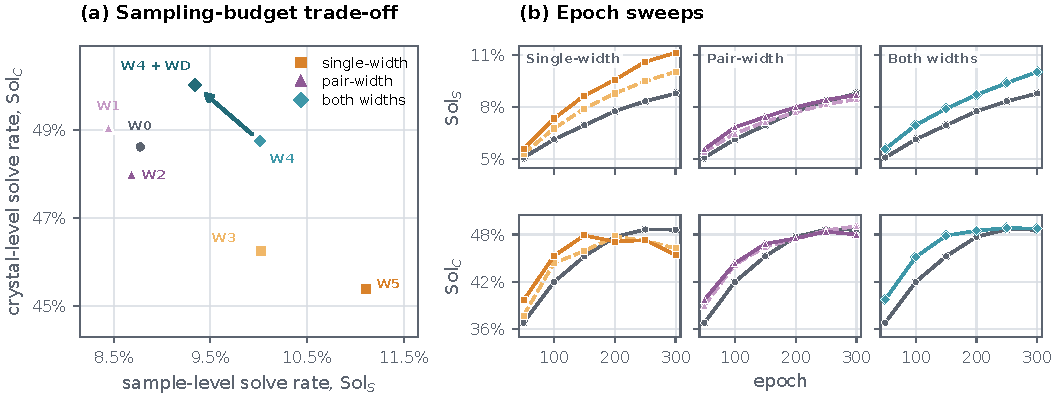
\includegraphics[width=\textwidth]{figures/generated/fig_width_scaling_tradeoff.pdf}
  \caption{\textbf{Balanced width scaling reaches the sampling-budget Pareto
    frontier.} \textbf{(a)} Single-sample solve rate
    $\mathrm{Sol}_S$ ($k{=}1$) versus crystal-level solve rate
    $\mathrm{Sol}_C$ at $k{=}30$ at epoch 300. Marker shape and color indicate the
    width-scaling family. Scaling either the single or pair width alone does not
    consistently improve the trade-off between per-sample success and target
    coverage, whereas jointly scaling both widths reaches the Pareto frontier.
    Adding weight decay of $10^{-2}$ further shifts the balanced model toward
    higher $k{=}30$ coverage. W0 is selected as \model{}-M, and W4 with weight
    decay (W4 + WD) as \model{}-L. \textbf{(b)} Epoch sweeps for single-width
    scaling (W0, W3, W5), pair-width scaling (W0, W1, W2), and balanced scaling
    (W0, W4). Top and bottom rows report $\mathrm{Sol}_S$ and $\mathrm{Sol}_C$,
    respectively. All metrics use the shared validation protocol with 30
    candidates per target and 200-step EDM--Heun sampling.}
  \label{fig:width-scaling-tradeoff}
\end{figure}